\chapter{Implementation, Training and Results}

\section{Software Organization}
The source code is available in the repository in the following locations:
\begin{itemize}
\item \texttt{src/amc/data.py}: RadioML loading, normalization, and splits.
\item \texttt{src/amc/model.py}: Phase 1 CNN baseline.
\item \texttt{src/amc/communications.py}: modulation, channel, estimation,
      equalization, and demodulation.
\item \texttt{scripts/train.py}: Phase 1 CNN training.
\item \texttt{scripts/evaluate.py}: Phase 1 evaluation.
\item \texttt{scripts/run\_phase2\_link.py}: complete Phase 2 link experiment.
\item \texttt{scripts/build\_parameter\_figures.py}: report figures and
      parameter records.
\end{itemize}

\section{Phase 1 CNN Training}
The baseline contains three Conv1D blocks with 64, 128, and 256 filters,
batch normalization, ReLU, max-pooling, adaptive average pooling, dropout,
and an 11-class output layer. It has 144,331 trainable parameters. Training
uses class-weighted cross-entropy, AdamW, cosine annealing, learning rate
$3\times10^{-4}$, weight decay $10^{-4}$, batch size 1024, seed 42, and
eight reported epochs.

\begin{figure}[H]
\centering
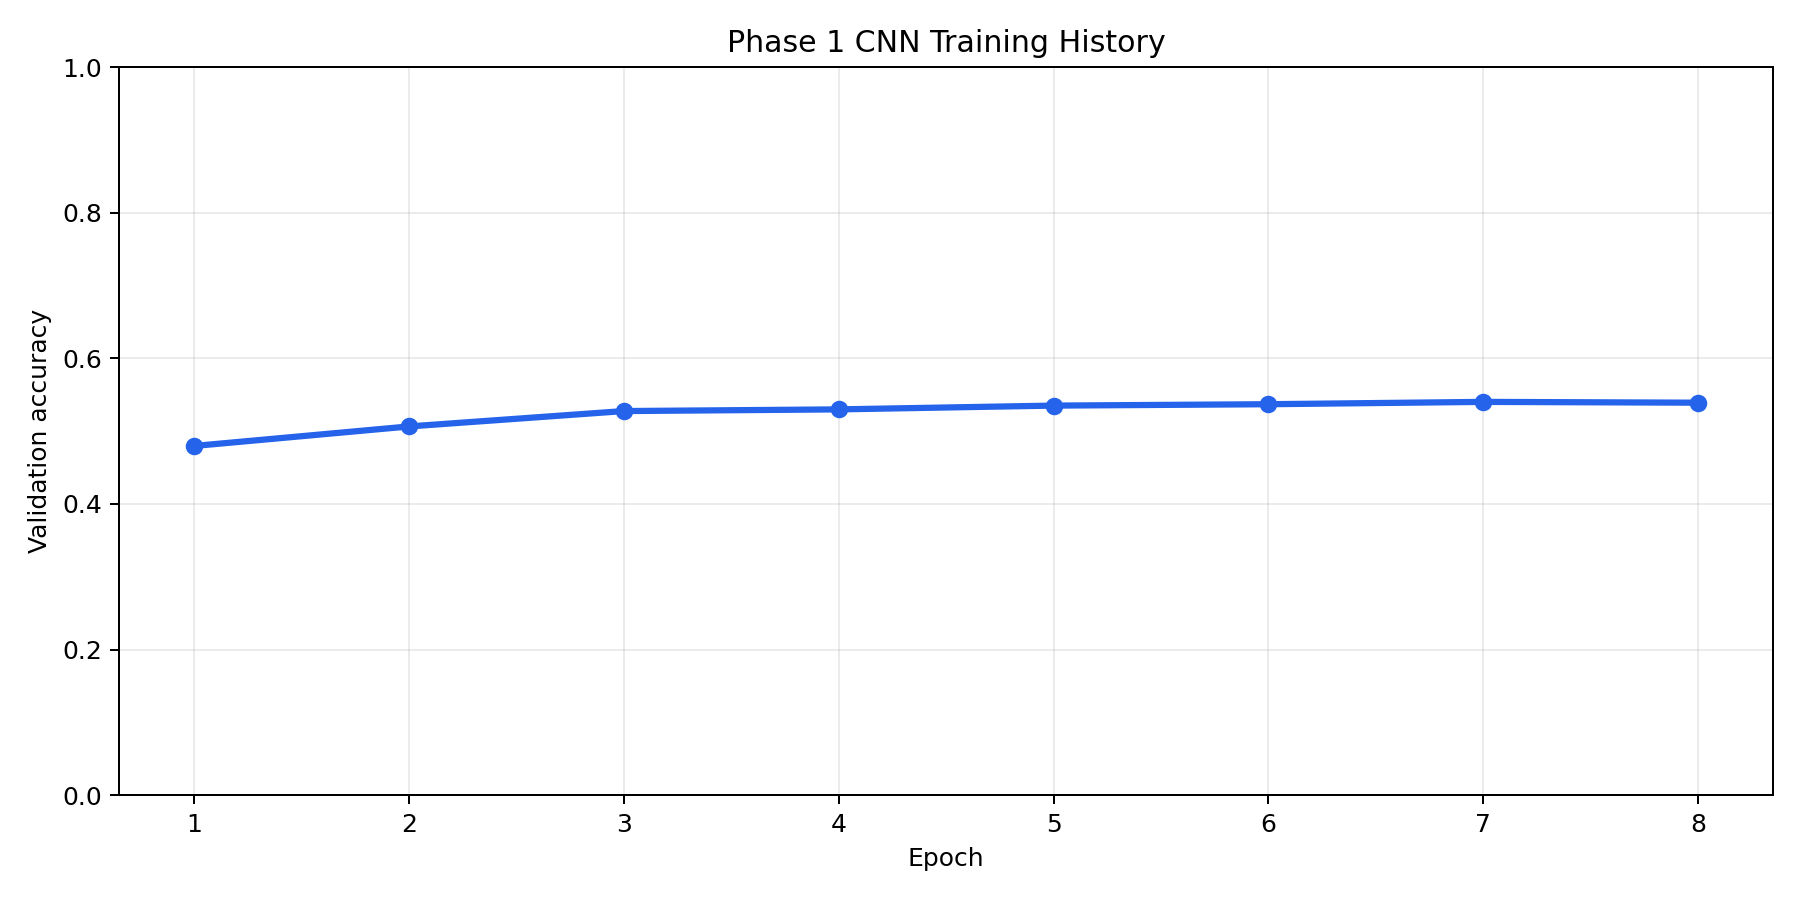
\includegraphics[width=0.9\textwidth]{artifacts/phase1-training-history.png}
\caption{Phase 1 CNN validation accuracy history.}
\label{fig:training}
\end{figure}

\section{Phase 2 Configuration}
\begin{table}[H]
\centering
\caption{Phase 2 experiment parameters.}
\begin{tabular}{p{6cm} p{7cm}}
\hline
\textbf{Parameter} & \textbf{Value}\\
\hline
Modulations & BPSK, QPSK, 8-PSK, 16-QAM\\
Frame length & 256 symbols\\
Channel & Block Rayleigh fading and AWGN\\
Impairments & Phase and frequency offset\\
SNR sweep & -4 to +16 dB, 2 dB step\\
Frames per SNR & 200\\
Metrics & BER, SER, decision accuracy, packet success, throughput\\
Random seed & 42\\
\hline
\end{tabular}
\end{table}

\section{Execution}
From the repository root, install the dependencies and execute:
\begin{verbatim}
python scripts/run_phase2_link.py --frames 200 \
  --output artifacts/phase2-link-results.png
\end{verbatim}
The command generates a PNG graph and a JSON result file. The final
comparison figure is generated using:
\begin{verbatim}
python scripts/build_final_report.py
\end{verbatim}

\section{Phase 1 Results}
The Phase 1 CNN achieved 53.94\% accuracy on 33,000 held-out RadioML
examples. Accuracy increased from 9.24\% at -20 dB SNR to 81.68\% at +12 dB.

\begin{figure}[H]
\centering
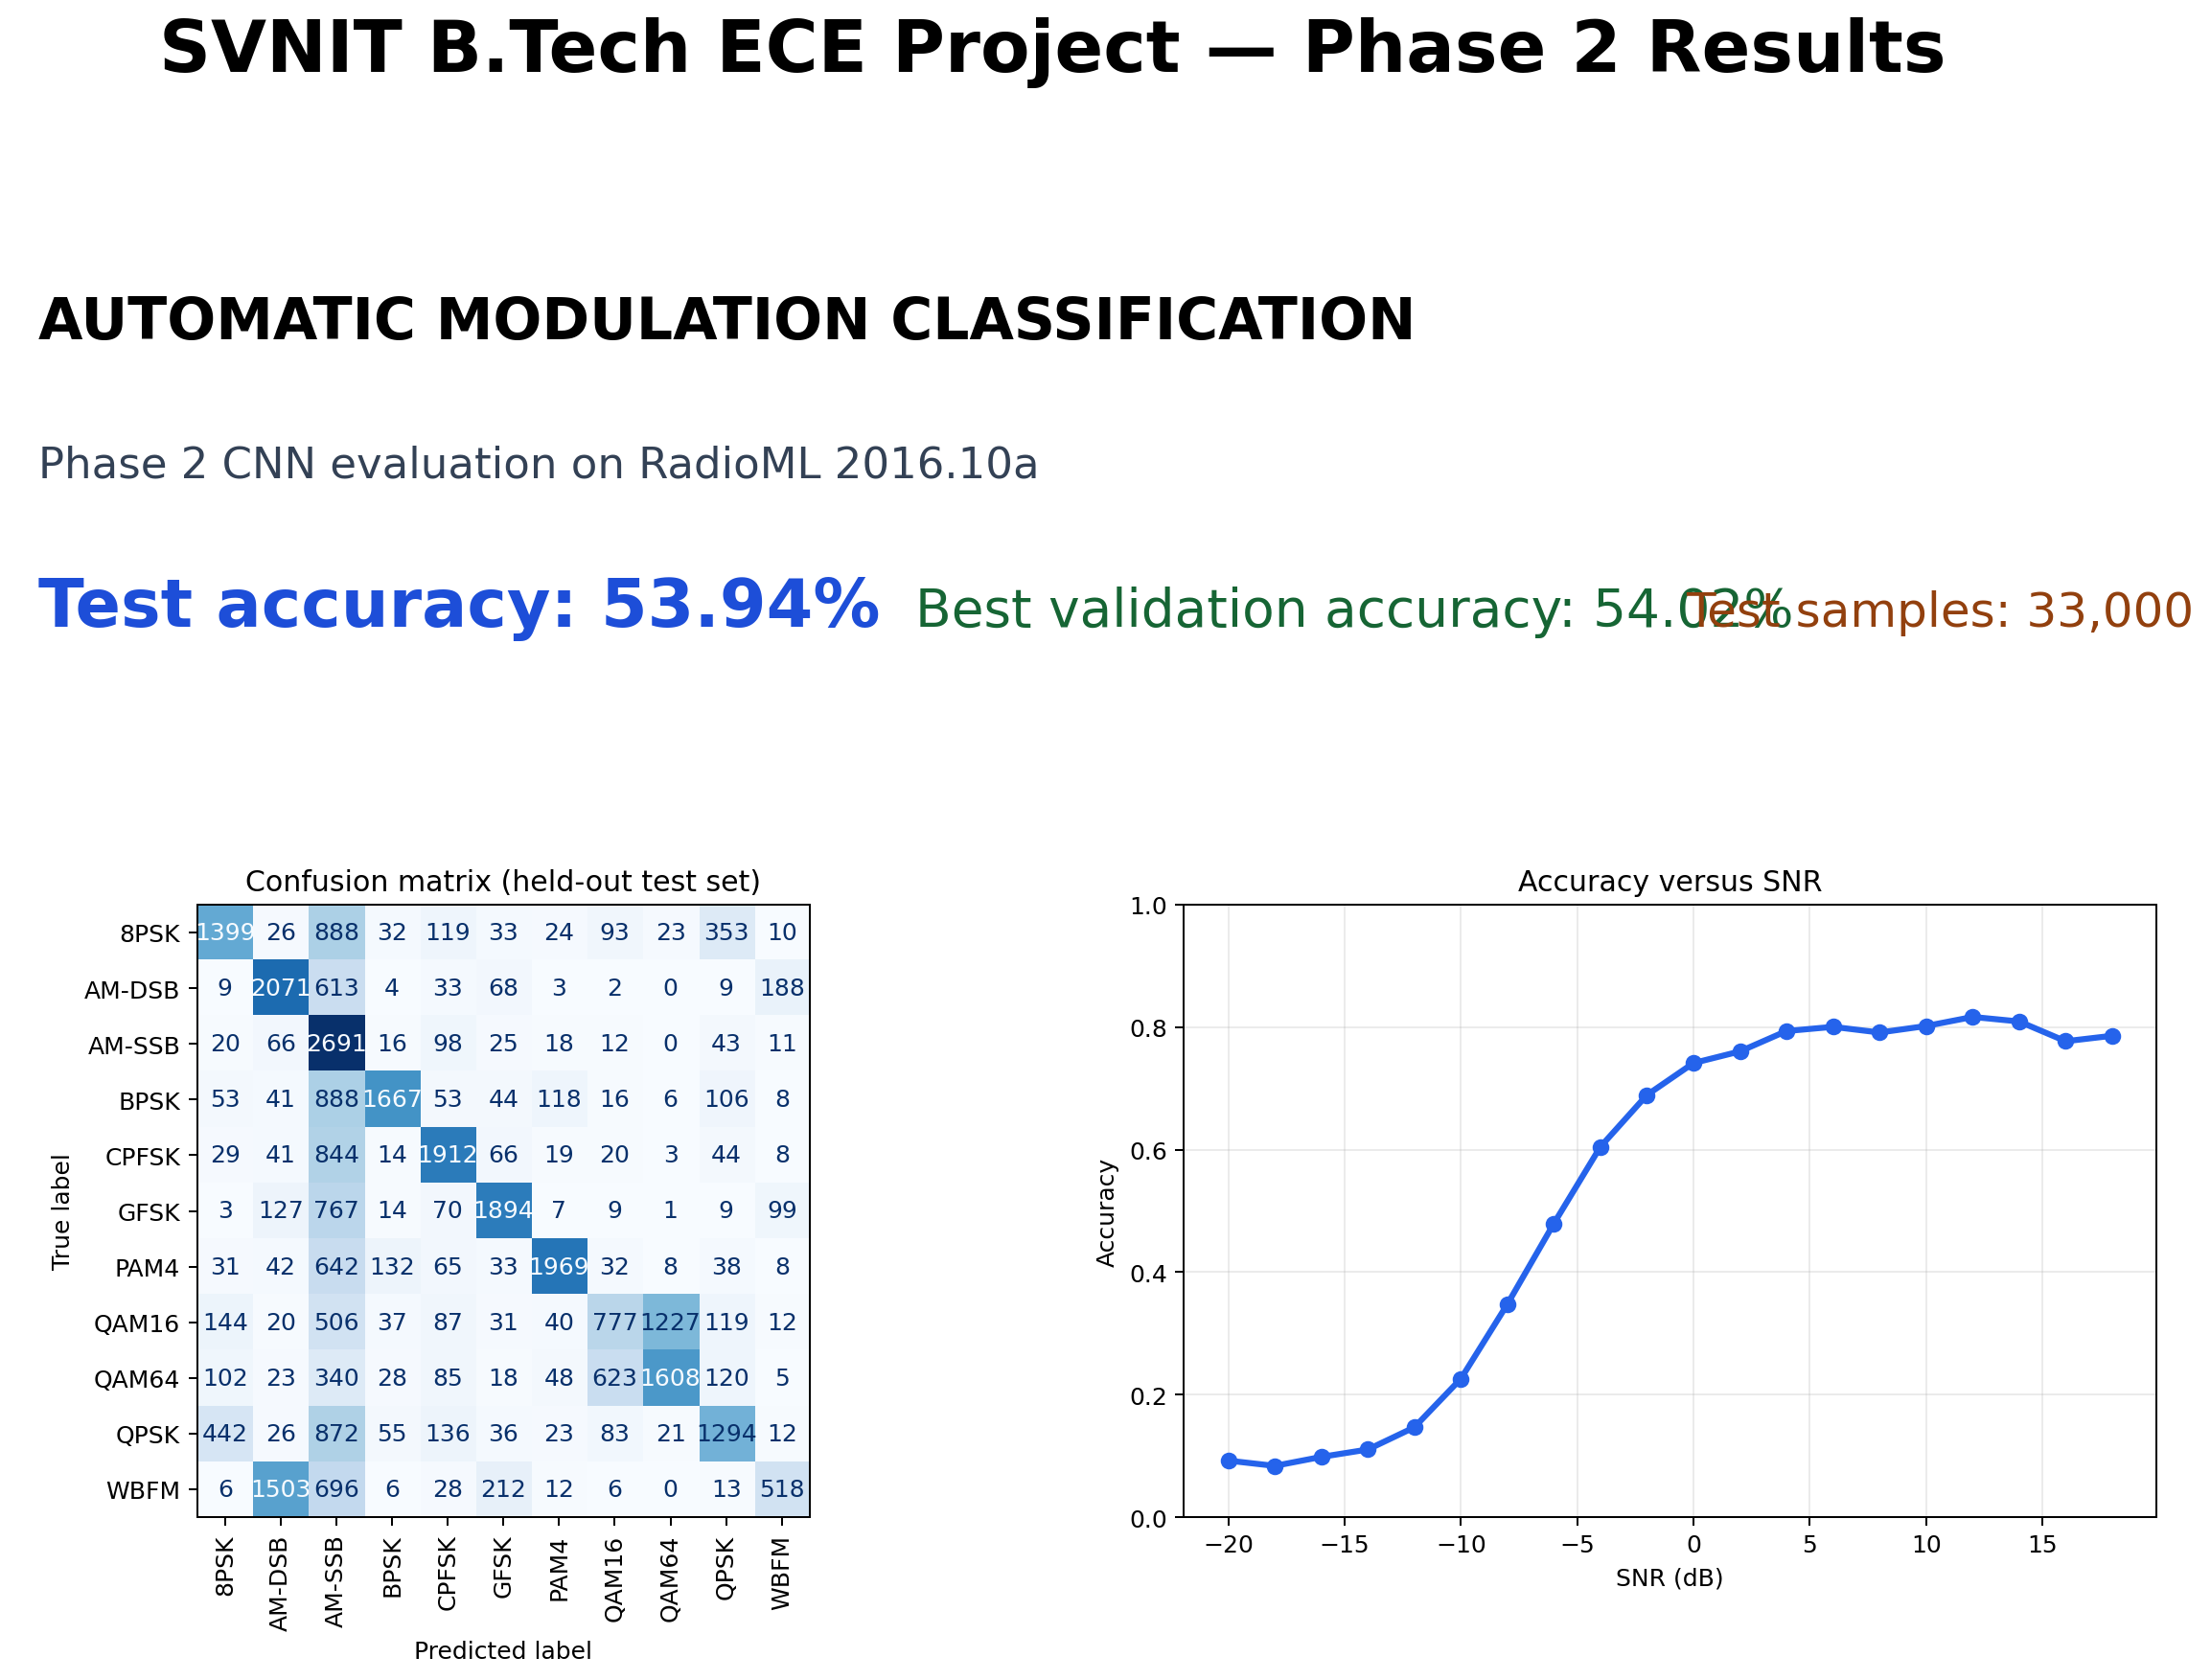
\includegraphics[width=\textwidth]{artifacts/phase2-results.png}
\caption{Phase 1 confusion matrix and SNR-wise accuracy.}
\label{fig:phase1}
\end{figure}

\section{Phase 2 Results}
At 10 dB, the adaptive receiver achieved 4.69\% BER, 6.94\% SER, 99.5\%
modulation-decision accuracy, and 49.0\% packet success. At 16 dB, it
achieved 0.095\% BER, 0.172\% SER, 100\% decision accuracy, 75.5\% packet
success, and 1.888 bits/symbol effective throughput.

\begin{figure}[H]
\centering
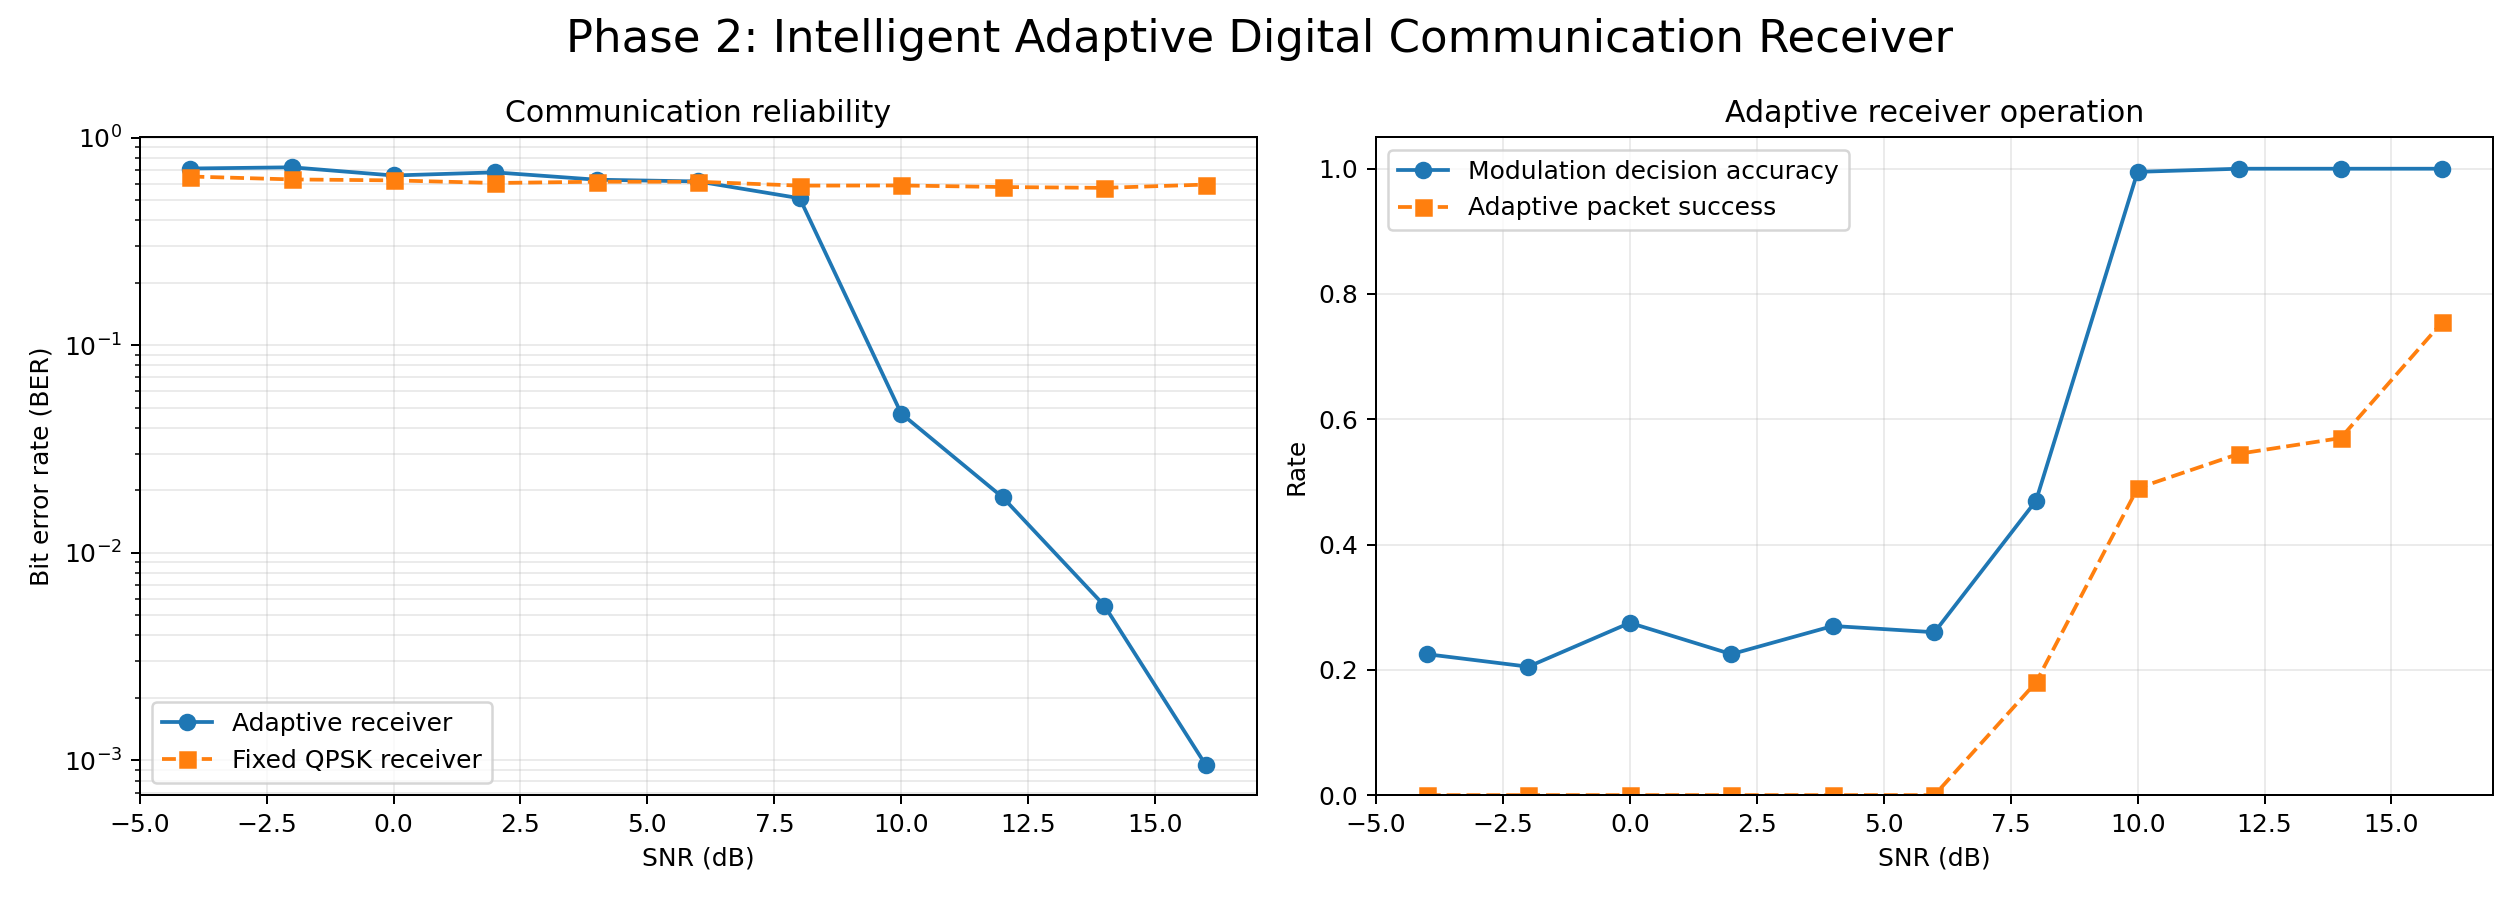
\includegraphics[width=\textwidth]{artifacts/phase2-link-results.png}
\caption{Phase 2 BER, SER, decision accuracy, packet success, and throughput.}
\label{fig:phase2}
\end{figure}

\section{Phase 1 versus Phase 2}
\begin{table}[H]
\centering
\caption{Comparison of the two project phases.}
\begin{tabular}{p{5cm} p{4cm} p{4cm}}
\hline
\textbf{Aspect} & \textbf{Phase 1} & \textbf{Phase 2}\\
\hline
Objective & Classify modulation & Operate adaptive receiver\\
Input & Fixed labeled dataset & Generated communication frames\\
Output & Class label & Recovered bits and link metrics\\
Channel & Dataset conditions & AWGN, Rayleigh, phase/frequency offsets\\
Receiver action & No demodulator control & Automatic demodulator selection\\
Main result & 53.94\% accuracy & 0.095\% BER at 16 dB\\
\hline
\end{tabular}
\end{table}

\begin{figure}[H]
\centering
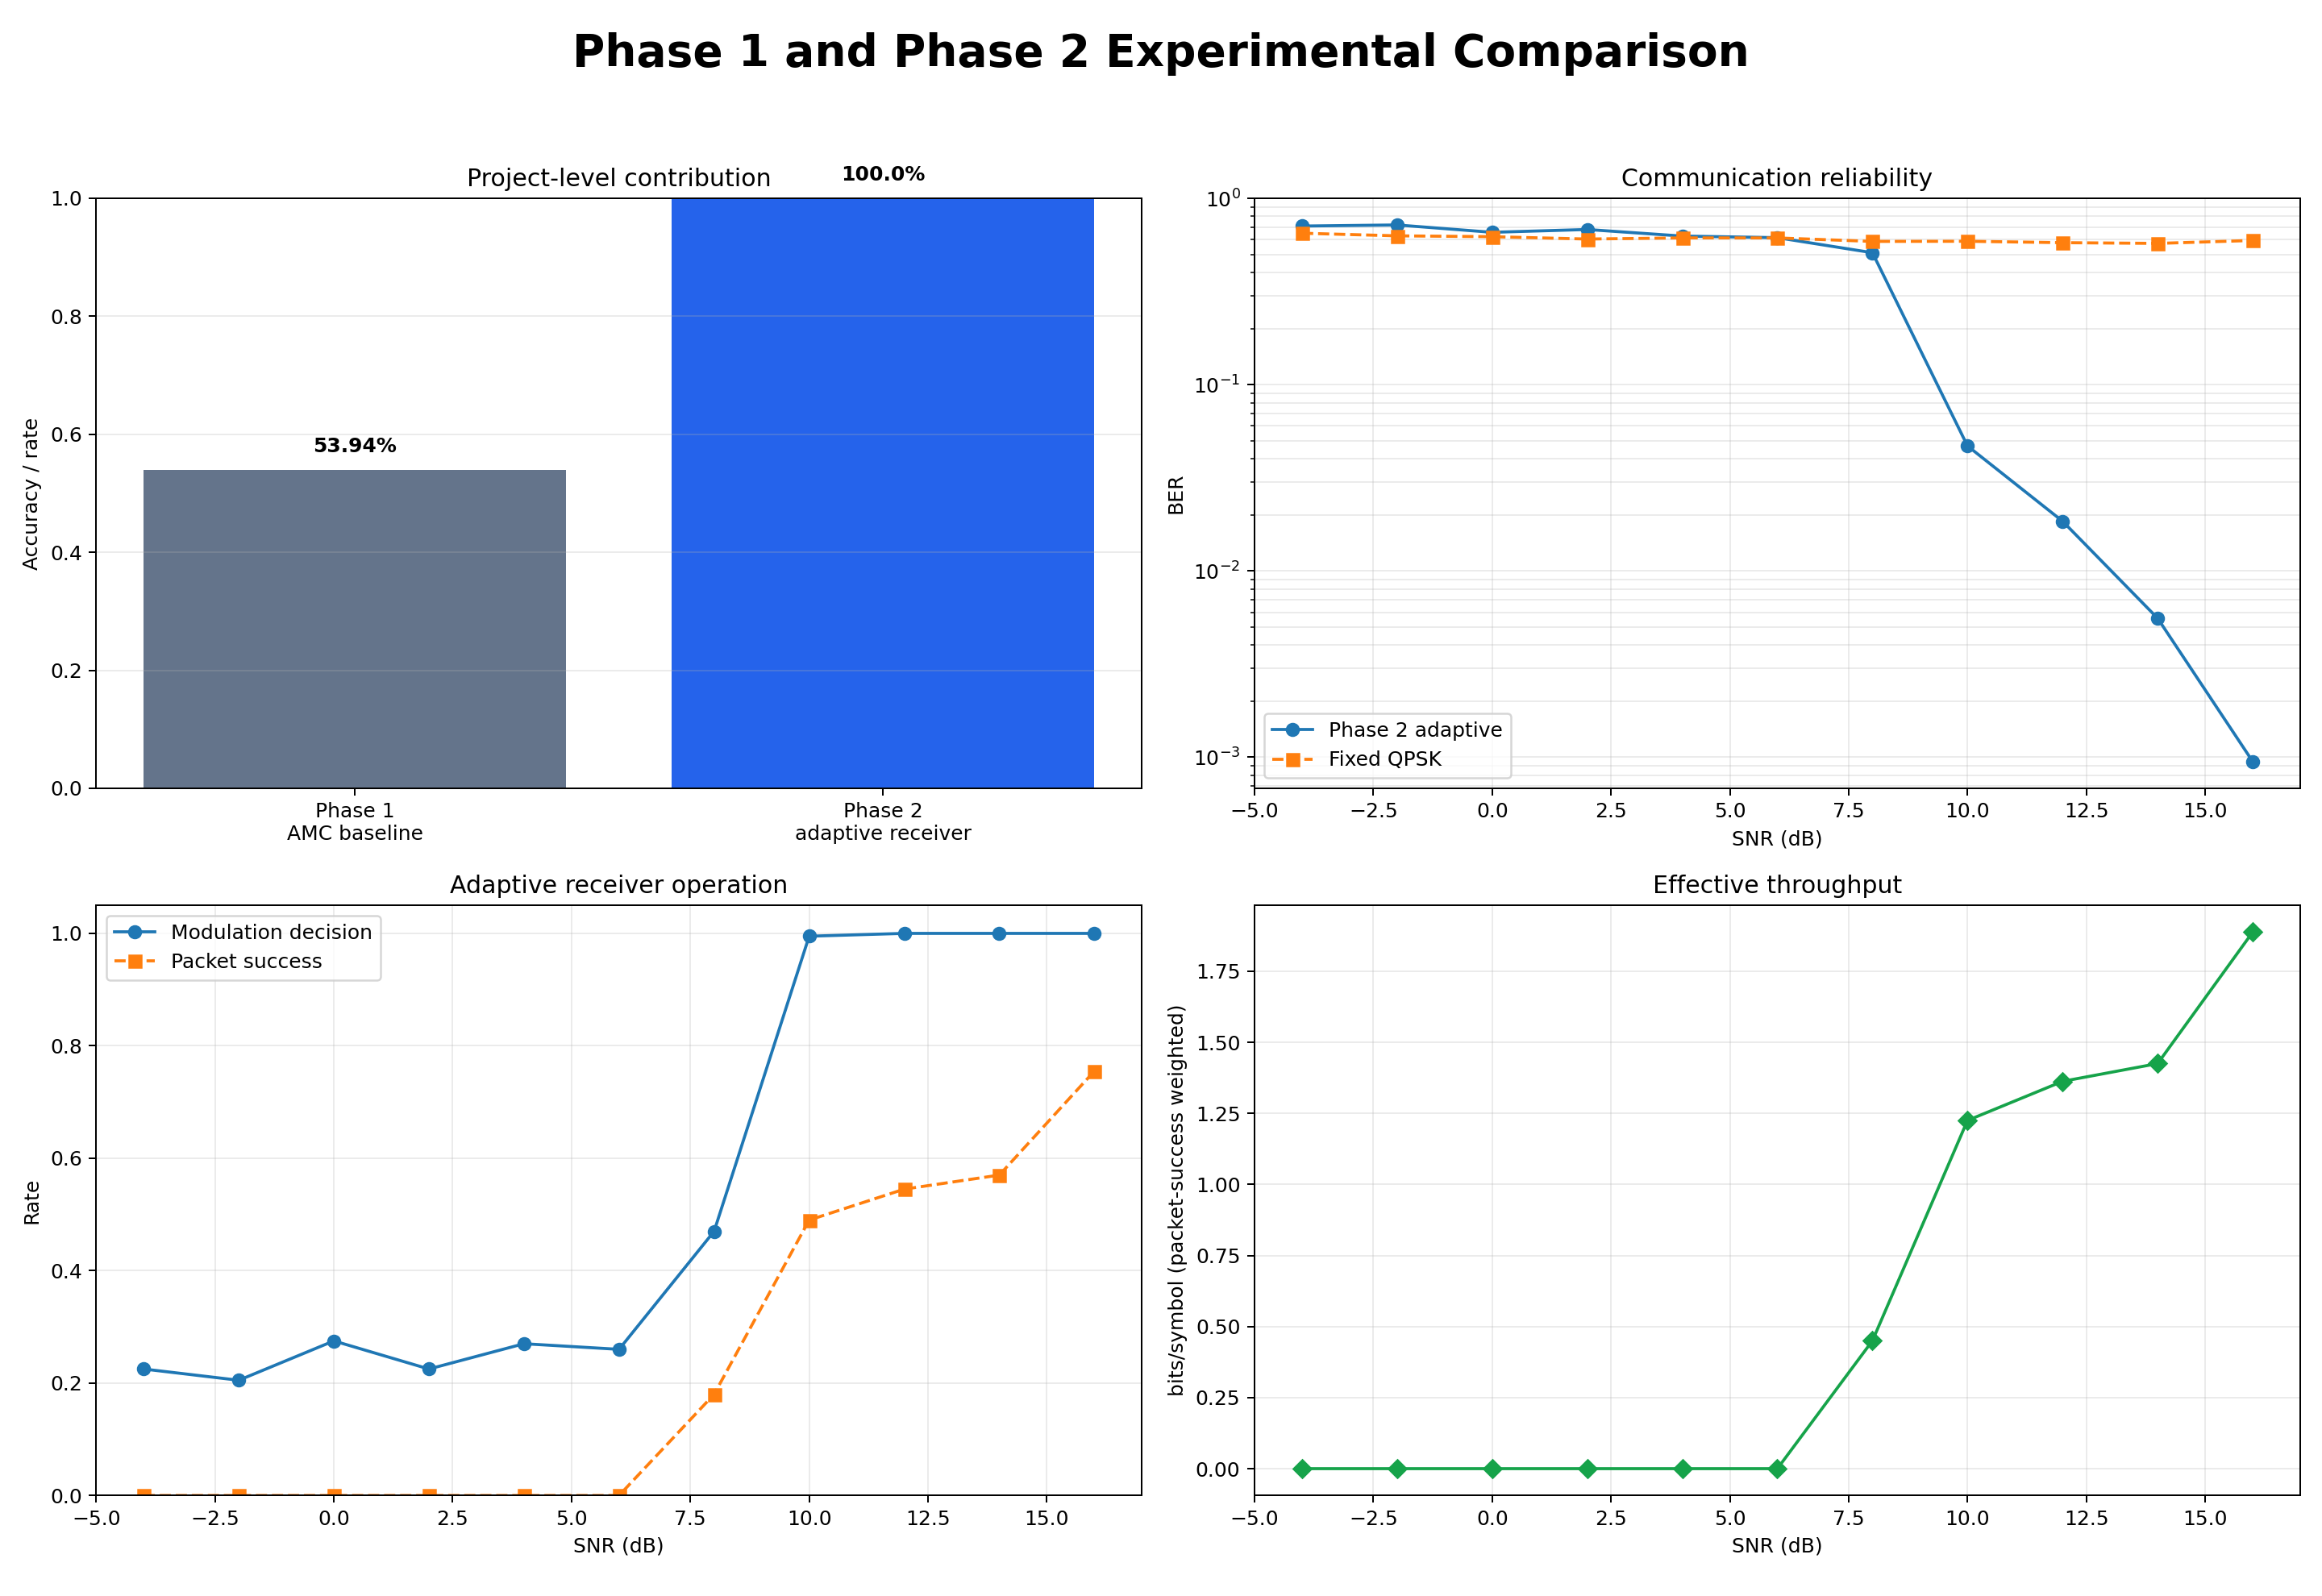
\includegraphics[width=\textwidth]{artifacts/final-phase1-phase2-comparison.png}
\caption{Consolidated Phase 1 and Phase 2 comparison.}
\label{fig:comparison}
\end{figure}

\section{Limitations}
The experiment is a controlled software simulation. Channel correction is
pilot-assisted, and the current link estimator is constellation-based rather
than an online neural classifier. Pulse shaping, coding, timing loops,
automatic gain control, and over-the-air SDR validation remain future work.
